% Setup the document.
\documentclass[11pt]{report}

% Import package used in the document.
\usepackage{er-ug}
\usepackage{er-abbrev}
\usepackage{er-math}
\usepackage{er-outline}

\usepackage{upquote}

% Setup the outline package.
\setboolean{showOutline}{false}

% Load any abbreviations.
\input{abbreviations}

% Start the document.
\begin{document}

% Set the page numbering to be lowercase roman numerals for the front matter.
\newpage
\singlespacing
\normalsize
\setcounter{page}{1}
\renewcommand{\thepage}{\roman{page}}

% Title page.
\thispagestyle{empty}
\begin{center}{
\vspace*{0.85in}
{\huge Lattice Microbes User's Guide}\\
\vspace*{0.5in}
{\large Version 2.0}\\
{\large \today}\\
\vspace*{0.9in}
{\large Authors:}\\
{\large Elijah Roberts}\\
{\large Zan Luthey-Schulten}\\
~\\
{\large Luthey-Schulten Group}\\
{\large University of Illinois at Urbana-Champaign}\\
{\large http://www.scs.illinois.edu/schulten/}\\
{\large http://latticemicrobes.sourceforge.net/}\\
\vspace*{1.45in}
{\Large Description}\\
}\end{center}

The Lattice Microbes User's Guide describes how to use the software to perform and analyze stochastic simulations of spatially modeled microbial cells. Lattice Microbes development is supported by the Department of Energy Office of Science (BER) under grant DE-FG02-10ER6510. 

% Table of contents
\newpage
\tableofcontents

% List of tables
\newpage
\addcontentsline{toc}{chapter}{List of Tables}
\listoftables

% List of figures
\newpage
\addcontentsline{toc}{chapter}{List of Figures}
\listoffigures

% List of abbreviations
%\newpage
%\addcontentsline{toc}{chapter}{List of Abbreviations}
%\listofabbreviations

% Set the page numbering to be arabic numerals for the text.
\newpage
\setcounter{page}{1}
\renewcommand{\thepage}{\arabic{page}}

% Main text.
\chapter{Quick-Start Guide}

\section{Simulating a bimolecular reaction}

As a simple first example, we will consider the reversible bimolecular reaction $A + B \xrightleftharpoons[k_{2}]{k_{1}} C$. We will simulate two variations of this reaction, one it which the molecules are assumed to move very quickly relative to the reaction rate (``well-stirred'') and one in which the diffusion rates do play a significant role in the reacting system. We will solve these two models using \abr{CME} and \abr{RDME} sampling methods, respectively.\\

The overall steps involved will be as follows:
\begin{enumerate}
\item Build the simulation files containing the reaction and diffusion models.
\item Run the simulations using any solver specific parameters.
\item Analyze the simulation output. Output is saved directly into the simulation file.
\end{enumerate}

To begin, open a terminal and change to the \file{qs/bimol} directory in your User's Guide installation.

\subsection{Building the models}

The most straightforward way to construct a reaction model for a Lattice Microbes simulation is to directly set the matrices in the simulation file. The utilities \file{lm\_setrm} and \file{lm\_setdm} allow one to set the matrices for the reaction and diffusion models, respectively. The details of the matrices themselves will be described elsewhere. For the bimolecular reaction described above with $k1=\scimath{1.07}{5}\,M^{-1}\,s^{-1}$ and $k2=0.351\,s^{-1}$, we use the following command to build the reaction model:
{\small\begin{verbatim}
[user@host qs/bimol]$ lm_setrm bimol-cme.lm numberSpecies=3 numberReactions=2 \
                    "InitialSpeciesCounts=[1000,1000,0]" "ReactionTypes=[2,1]" \
                    "ReactionRateConstants(:,0)=[1.78e-4;0.351]" \
                    "StoichiometricMatrix=[-1,1;-1,1;1,-1]" \
                    "DependencyMatrix=[1,0;1,0;0,1]"
\end{verbatim}}

Note that we used the relationship between the stochastic and deterministic second order rate constants $k2'=k2/N_A{\cdot}V$ with a simulation volume of $V=\scimath{1}{-15}\,L$ to obtain the rate constant for the model. The file \file{bimol-cme.lm} is now ready to be simulated using the \abr{CME}.\\

Since the reaction portion of an \abr{RDME} model is identical to the \abr{CME} model, we simply copy the reaction model to a new simulation file and then set the diffusion matrices on the new file. Here, we use a diffusion coefficient $D=\scimath{1}{-14}\,m^2\,s{-1}$ for all molecules and a $32{\times}32{\times}32$ lattice with a spacing of $\lambda=\scimath{31.25}{-9}\,m$.
{\small\begin{verbatim}
[user@host qs/bimol]$ cp bimol-cme.lm bimol-rdme.lm
[user@host qs/bimol]$ lm_setdm bimol-rdme.lm numberReactions=2 numberSpecies=3 \
                    numberSiteTypes=1 "latticeSize=[32,32,32]" \
                    latticeSpacing=31.25e-9 particlesPerSite=8 \
                    "DiffusionMatrix=[1e-14]" "ReactionLocationMatrix=[1]"
\end{verbatim}}

The file \file{bimol-rdme.lm} is now ready to be simulated using the \abr{RDME}.

\subsection{Running the simulations}

\subsubsection{Sampling the CME using the Gillespie direct method}

To simulate the well-stirred version of the bimolecular reaction model, we will use the Gillespie direct method, which is the default method for well-stirred simulations in Lattice Microbes. Before we run the simulations, we first set a few simulation parameters for the solver. The \file{lm\_setp} utility allows one to set solver specific parameters in the simulation file. Here, we tell the solver to simulate for 10 seconds and write out the system state every 0.001 second.
{\small\begin{verbatim}
[user@host qs/bimol]$ lm_setp bimol-cme.lm writeInterval=1e-3 maxTime=1e1
\end{verbatim}}

Finally, we run the actual simulation itself:
{\small\begin{verbatim}
[user@host qs/bimol]$ lm -r 1-100 -ws -f bimol-cme.lm
\end{verbatim}}
The \file{-r} option tells the solver to simulate replicates 1--100 and the \file{-ws} option tells Lattice Microbes to use the default well-stirred solver. Following completion of the runs the \file{bimol-cme.lm} file will contain the sampling data for all of the simulation replicates.

\subsubsection{Sampling the RDME using the next-subvolume method}

If no \abrs{GPU} are attached to your computer, the only available \abr{RDME} solver is the next-subvolume method. We first set the appropriate parameters as before, but additionally, since we wish to track individual molecules, we must set a lattice output interval. Writing the lattice too frequently can consume an enormous amount of disk space so one should sample the lattice much less frequently than the system state, which only outputs the total count of each molecule type. Here, we sample the lattice every 0.1 second so we will have 100 samples of each 10 second simulation replicate.
{\small\begin{verbatim}
[user@host qs/bimol]$ lm_setp bimol-rdme.lm writeInterval=1e-3 \
                    latticeWriteInterval=1e-1 maxTime=1e1
\end{verbatim}}

We then run the \abr{RDME} simulations. These simulations take significantly longer than the well-stirred equivalents, so here we only simulate 10 replicates:
{\small\begin{verbatim}
[user@host qs/bimol]$ lm -r 1-10 -sl lm::rdme::NextSubvolumeSolver \
                    -f bimol-rdme.lm
\end{verbatim}}

All of the system state information and lattice data for every replicate will be saved into the \file{bimol-cme.lm} file.

\subsubsection{Sampling the RDME using the MPD-RDME method}

If you do have an NVIDIA \abr{GPU} attached to your computer, you can also use the MPD-RDME solver. This is an approximate RDME solver that uses a time stepping approach to dramatically increase simulation performance. We will run ten additional RDME replicates using the MPD-RDME. First, set the time step parameter to 3 milliseconds:
{\small\begin{verbatim}
[user@host qs/bimol]$ lm_setp bimol-rdme.lm timestep=3.0e-3
\end{verbatim}}

Then run replicates 11-20 using the MPD-RDME solver:
{\small\begin{verbatim}
[user@host qs/bimol]$ lm -r 11-20 -sl lm::rdme::MpdRdmeSolver -f bimol-rdme.lm
\end{verbatim}}

Following completion of the runs, ten additional simulation replicates will have been added to the \file{bimol-cme.lm} file.

\subsection{Looking at the simulation output}

\begin{figure}
\centerline{\includegraphics[width=4in]{Tutorials/HDFViewOpen.png}}
\caption{HDFView showing an open Lattice Microbes simulation file.}
\label{fig:HDFViewOpen}
\end{figure}

The output data is stored in a Lattice Microbes simulation file, which is an HDF5 encoded file that stores large, independent data sets in a hierarchical structure. To view the data, one must use an HDF5 viewer such as HDFView available at:\\
\url{http://www.hdfgroup.org/hdf-java-html/hdfview/}\\

To install the HDFView program, please follow the installation instructions for your platform.

\subsubsection{Opening a simulation file}

To open a Lattice Microbes simulation file in HDFView choose \gui{File$\rightarrow$Open} from the menu. Navigate to your \file{qs/bimol} directory in the \gui{Open} dialog. Be sure to change the \gui{Files of Type:} option to \gui{All Files} and then select the \file{bimol-cme.lm} file.\\

Once the file is opened, the individual folders containing the \gui{Model}, \gui{Parameters}, and \gui{Simulation} data can be expanded, as shown in \Figure{fig:HDFViewOpen}. Datasets are shown as small grid-like icons underneath the folders. Double clicking on a dataset will display its contents in the viewer panel to the right. For additional usage details, please see the HDFView User's Guide, located on the download page given above.


\subsubsection{Overview of the file format}

Lattice Microbes simulation files are organized into three top level folders: \gui{Model}, \gui{Parameters}, and \gui{Simulation}.\\

The \gui{Model} folder contains two subfolders for the \gui{Reaction} and \gui{Diffusion} models, as needed for the simulation. Each folder has several attributes and contains several datasets corresponding to the matrices that describe the model. Further details of the matrices themselves are provided elsewhere.\\

The \gui{Parameters} folder acts as a collection point for solver specific parameters, which are set as attributes on the folder. Details of individual parameters are provided elsewhere.\\

The \gui{Simulations} folder contains the actual output from the simulations. Beneath the folder is one folder for each simulation replicate, numbered accordingly. For each simulation replicate the data is stored in a variety of matrices and folders, which are specific to the simulation method.

\subsection{Analyzing a simulation using Matlab}

The HDF5 file format used by the Lattice Microbes software can be directly read by Matlab, easing the analysis of simulation data. Here, we will calculate the probability as a function of time for the system to have a specific number of A molecules, {\ie}, $P_A(t)$. We will use this \abr{PDF} to calculate the mean and variance as a function of time.\\

First, we load the number of A molecules for each replicate at each time point from the simulation file and transform the counts into a \abr{PDF}:
{\small\begin{verbatim}
inputFilename='bimol-cme.lm';
x=[0:1000];
numberReplicates=100;
species=1;
for R=[1:numberReplicates]
    if R == 1
        ts=cast(permute(hdf5read(inputFilename,...
           sprintf('/Simulations/%07d/SpeciesCountTimes',R)),[2,1]),'double');
        Pt=zeros(size(x,2),size(ts,2));
    end
    counts=cast(permute(hdf5read(inputFilename,...
           sprintf('/Simulations/%07d/SpeciesCounts',R)),[2,1]),'double');
    for ti=[1:size(ts,2)]
        Pt(counts(ti,species)+1,ti)=Pt(counts(ti,species)+1,ti)+1;
    end
end
Pt=Pt./numberReplicates;
\end{verbatim}}

Note that HDF5 files store data in row major format while Matlab stores data in column major format. In the above Matlab code, we used the \file{permute(hdf5read(...),[2,1])} command to reorder the 2D matrices to column major format after the data was loaded.\\

Next, we calculate the mean and variance from the $P_A(t)$:
{\small\begin{verbatim}
E=zeros(1,size(ts,2));
V=zeros(1,size(ts,2));
for ti=[1:size(ts,2)]
    E(ti)=sum(x'.*Pt(:,ti));
    V(ti)=sum((power(x'-E(ti),2)).*Pt(:,ti));
end
\end{verbatim}}

Finally, we plot the mean and variance as a function of time:
{\small\begin{verbatim}
subplot(2,1,1);
plot(ts(1:10:end), E(1:10:end));
axis([0 10 1e2 1e3]); xlabel('Time (s)'); ylabel('E\{A(t)\}');
subplot(2,1,2);
plot(ts(1:10:end), V(1:10:end));
axis([0 10 1e0 2e2]); xlabel('Time (s)'); ylabel('Var\{A(t)\}');
\end{verbatim}}

\begin{figure}
\centerline{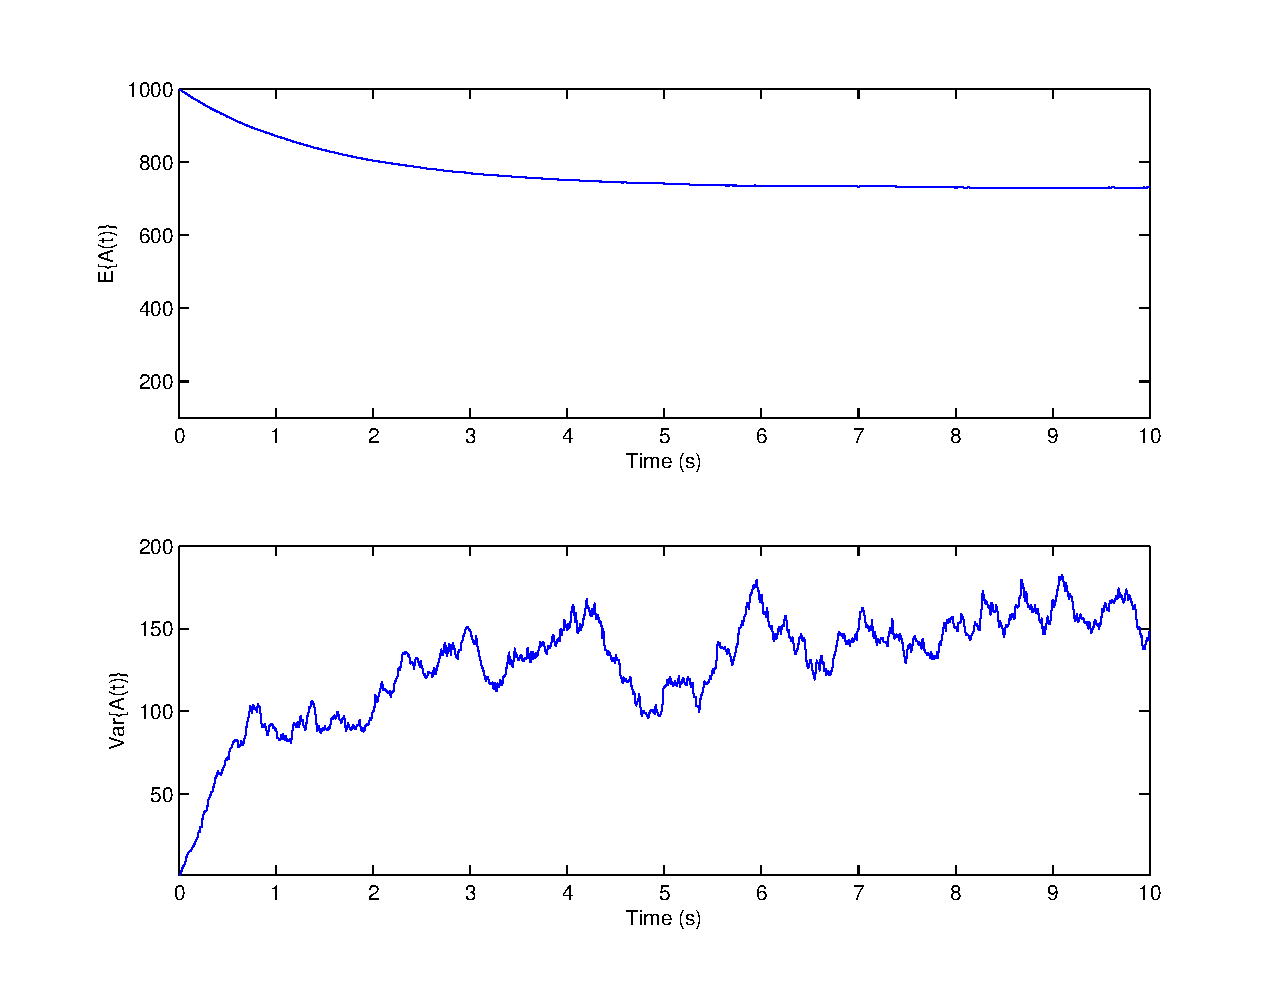
\includegraphics[width=6in]{Tutorials/MatlabPlot.eps}}
\caption{Mean and variance of A(t) for the reaction $A + B \xrightleftharpoons[]{} C$.}
\label{fig:MatlabPlot}
\end{figure}

The resulting plot should look like that shown in \Figure{fig:MatlabPlot}.\\

As another example, we calculate some statistics about the distribution of the molecules in \abr{RDME} simulations. The lattice is stored as a four dimensional matrix with dimensions $x{\times}y{\times}z{\times}particlesPerSite$. In our example above, the number of particles per site was limited to eight. We will count the number of particles in any sites' first, second, third, etc position. Such a calculation can give an indication of how close the lattice is to overflowing.

{\small\begin{verbatim}
replicate=1;
L=permute(h5read('bimol-rdme.lm',sprintf('/Model/Diffusion/Lattice')),[4,3,2,1]);
psum=sum(sum(sum(L>0)));
disp(sprintf('initial=%d (%d %d %d %d %d %d %d %d) %d--%d',...
             sum(sum(sum(sum(L>0)))),psum,min(min(min(min(L)))),...
             max(max(max(max(L))))));
for ts=[0:100]
    L=permute(h5read('bimol-rdme.lm',...
             sprintf('/Simulations/%07d/Lattice/%010d',...
             replicate,ts)),[4:-1:1]);
    psum=sum(sum(sum(L>0)));
    disp(sprintf('ts %4d=%d (%d %d %d %d %d %d %d %d) %d--%d',ts,...
             sum(sum(sum(sum(L>0)))),psum,min(min(min(min(L)))),...
             max(max(max(max(L))))));
end
\end{verbatim}}

Note that here again we used the \file{permute(hdf5read(...),[4,3,2,1])} command to reorder the 4D matrices to column major format after the data was loaded.\\

\subsection{Visualizing a trajectory using VMD}

If you have installed the VMD plugin, you can use VMD to visualize \abr{RDME} trajectories. For general instructions on using VMD, please see the VMD help at \url{http://www.ks.uiuc.edu/Research/vmd/}. Here we will focus on using VMD to visualize Lattice Microbes trajectories. First, ensure that your VMD plugin is functioning by starting VMD and then checking the VMD console for a message like:

{\small\begin{verbatim}
LMplugin Info) version 2 build by XXXXXXXX on XXX at XXXX-XX-XX XX:XX:XX
\end{verbatim}}

\begin{figure}
\centerline{\includegraphics[width=4in]{Tutorials/VMDOpen.png}}
\caption{VMD open file dialog.}
\label{fig:VMDOpen}
\end{figure}

Next, go to the menu and choose \gui{File$\rightarrow$New Molecule...}. Select \gui{Lattice Microbes} in the \gui{Determine file type:} drop down and browse to the file \file{bimol-rdme.lm}. Finally, press the \gui{Load} button (see \Figure{fig:VMDOpen}).\\

The trajectory should load with 101 frames. Initially, the VMD \gui{OpenGL} display will show only small points for each molecule. Change the representation by choosing \gui{Graphics$\rightarrow$Representations...} from the menu and then changing the \gui{Drawing Method} drop down to be \gui{VDW}. Now the molecules should appear as spheres. Next, change the \gui{Coloring Method} drop down to be \gui{Type} and molecules of different types should appear in different colors, as shown in \Figure{fig:VMDMolecules}. Press the triangular play button to play the simulation trajectory.\\

\begin{figure}
\centerline{\includegraphics[width=4in]{Tutorials/VMDMolecules.png}}
\caption{VMD molecule display.}
\label{fig:VMDMolecules}
\end{figure}

Finally, you may use the \gui{Selected Atoms} text field in the \gui{Graphical Representations} dialog to change which molecules are displayed. Change the text from ``\file{all}'' to ``\file{name particle and type 1}'' to show only A molecules. Likewise you can use ``\file{name particle and type 2}'' and ``\file{name particle and type 3}'' to view molecules of type B and C respectively.




\subsection{Importing an SBML reaction model}

Finally, we will show how you can use SBML files to set the reaction model, in addition to specifying the reaction matrices as shown above. First, copy the following SBML text into a file named \file{bimol.sbml}

{\small\begin{verbatim}
<?xml version="1.0" encoding="UTF-8"?>
<sbml xmlns="http://www.sbml.org/sbml/level3/version1/core" level="3" version="1">
    <model id="bimolecular" substanceUnits="item" timeUnits="second"
           volumeUnits="litre" extentUnits="item">
        <listOfUnitDefinitions>
            <unitDefinition id="per_second">
                <listOfUnits>
                    <unit kind="second" exponent="-1" scale="0" multiplier="1"/>
                </listOfUnits>
            </unitDefinition>
            <unitDefinition id="per_item_per_second">
                <listOfUnits>
                    <unit kind="item"   exponent="-1" scale="0" multiplier="1"/>
                    <unit kind="second" exponent="-1" scale="0" multiplier="1"/>
                </listOfUnits>
            </unitDefinition>
            <unitDefinition id="per_molar_per_second">
                <listOfUnits>
                    <unit kind="litre"  exponent="1" scale="0" multiplier="1"/>
                    <unit kind="mole"   exponent="-1" scale="0" multiplier="1"/>
                    <unit kind="second" exponent="-1" scale="0" multiplier="1"/>
                </listOfUnits>
            </unitDefinition>
        </listOfUnitDefinitions>
        <listOfCompartments>
            <compartment id="cell" size="1e-15" spatialDimensions="3"
                         constant="true"/>
        </listOfCompartments>
        <listOfSpecies>
            <species id="A" compartment="cell" initialAmount="1000"
                     hasOnlySubstanceUnits="true" boundaryCondition="false"
                     constant="false"/>
            <species id="B" compartment="cell" initialAmount="1000"
                     hasOnlySubstanceUnits="true" boundaryCondition="false"
                     constant="false"/>
            <species id="C" compartment="cell" initialAmount="0"
                     hasOnlySubstanceUnits="true" boundaryCondition="false"
                     constant="false"/>
        </listOfSpecies>
        <listOfReactions>
            <reaction id="Forward" reversible="false" fast="false">
                <listOfReactants>
                    <speciesReference species="A" stoichiometry="1"
                                      constant="true"/>
                    <speciesReference species="B" stoichiometry="1"
                                      constant="true"/>
                </listOfReactants>
                <listOfProducts>
                    <speciesReference species="C" stoichiometry="1"
                                      constant="true"/>
                </listOfProducts>
                <kineticLaw>
                    <math xmlns="http://www.w3.org/1998/Math/MathML">
                        <apply>
                            <divide/>
                            <apply>
                                <times/>
                                <ci> k1 </ci>
                                <ci> A </ci>
                                <ci> B </ci>
                            </apply>
                            <apply>
                                <times/>
                                <csymbol encoding="text"
                      definitionURL="http://www.sbml.org/sbml/symbols/avogadro"/>
                                <ci> cell </ci>
                            </apply>
                        </apply>
                    </math>
                    <listOfLocalParameters>
                        <localParameter id="k1" value="1.07e5"
                                        units="per_molar_per_second"/>
                    </listOfLocalParameters>
                </kineticLaw>
            </reaction>
            <reaction id="Reverse" reversible="false" fast="false">
                <listOfReactants>
                    <speciesReference species="C" stoichiometry="1"
                    constant="true"/>
                </listOfReactants>
                <listOfProducts>
                    <speciesReference species="A" stoichiometry="1"
                                      constant="true"/>
                    <speciesReference species="B" stoichiometry="1"
                                      constant="true"/>
                </listOfProducts>
                <kineticLaw>
                    <math xmlns="http://www.w3.org/1998/Math/MathML">
                        <apply>
                            <times/>
                            <ci> k2 </ci>
                            <ci> C </ci>
                        </apply>
                    </math>
                    <listOfLocalParameters>
                        <localParameter id="k2" value="0.351" units="per_second"/>
                    </listOfLocalParameters>
                </kineticLaw>
            </reaction>
        </listOfReactions>
    </model>
</sbml>
\end{verbatim}}

Next, create a simulation file from the SBML file:
{\small\begin{verbatim}
[user@host qs/bimol]$ lm_sbml_import bimol-cme-sbml.lm bimol.sbml
\end{verbatim}}

The reaction model is now ready to be simulated:
{\small\begin{verbatim}
[user@host qs/bimol]$ lm_setp bimol-cme-sbml.lm writeInterval=1e-3 maxTime=1e1
[user@host qs/bimol]$ lm -r 1-100 -ws -f bimol-cme-sbml.lm
\end{verbatim}}


                                                               

\chapter{Quick-Start Guide}

\section{Simulating a bimolecular reaction}

As a simple first example, we will consider the reversible bimolecular reaction $A + B \xrightleftharpoons[k_{2}]{k_{1}} C$. We will simulate two variations of this reaction, one it which the molecules are assumed to move very quickly relative to the reaction rate (``well-stirred'') and one in which the diffusion rates do play a significant role in the reacting system. We will solve these two models using \abr{CME} and \abr{RDME} sampling methods, respectively.\\

The overall steps involved will be as follows:
\begin{enumerate}
\item Build the simulation files containing the reaction and diffusion models.
\item Run the simulations using any solver specific parameters.
\item Analyze the simulation output. Output is saved directly into the simulation file.
\end{enumerate}

To begin, open a terminal and change to the \file{qs/bimol} directory in your User's Guide installation.

\subsection{Building the models}

The most straightforward way to construct a reaction model for a Lattice Microbes simulation is to directly set the matrices in the simulation file. The utilities \file{lm\_setrm} and \file{lm\_setdm} allow one to set the matrices for the reaction and diffusion models, respectively. The details of the matrices themselves will be described elsewhere. For the bimolecular reaction described above with $k1=\scimath{1.07}{5}\,M^{-1}\,s^{-1}$ and $k2=0.351\,s^{-1}$, we use the following command to build the reaction model:
{\small\begin{verbatim}
[user@host qs/bimol]$ lm_setrm bimol-cme.lm numberSpecies=3 numberReactions=2 \
                    "InitialSpeciesCounts=[1000,1000,0]" "ReactionTypes=[2,1]" \
                    "ReactionRateConstants(:,0)=[1.78e-4;0.351]" \
                    "StoichiometricMatrix=[-1,1;-1,1;1,-1]" \
                    "DependencyMatrix=[1,0;1,0;0,1]"
\end{verbatim}}

Note that we used the relationship between the stochastic and deterministic second order rate constants $k2'=k2/N_A{\cdot}V$ with a simulation volume of $V=\scimath{1}{-15}\,L$ to obtain the rate constant for the model. The file \file{bimol-cme.lm} is now ready to be simulated using the \abr{CME}.\\

Since the reaction portion of an \abr{RDME} model is identical to the \abr{CME} model, we simply copy the reaction model to a new simulation file and then set the diffusion matrices on the new file. Here, we use a diffusion coefficient $D=\scimath{1}{-14}\,m^2\,s{-1}$ for all molecules and a $32{\times}32{\times}32$ lattice with a spacing of $\lambda=\scimath{31.25}{-9}\,m$.
{\small\begin{verbatim}
[user@host qs/bimol]$ cp bimol-cme.lm bimol-rdme.lm
[user@host qs/bimol]$ lm_setdm bimol-rdme.lm numberReactions=2 numberSpecies=3 \
                    numberSiteTypes=1 "latticeSize=[32,32,32]" \
                    latticeSpacing=31.25e-9 particlesPerSite=8 \
                    "DiffusionMatrix=[1e-14]" "ReactionLocationMatrix=[1]"
\end{verbatim}}

The file \file{bimol-rdme.lm} is now ready to be simulated using the \abr{RDME}.

\subsection{Running the simulations}

\subsubsection{Sampling the CME using the Gillespie direct method}

To simulate the well-stirred version of the bimolecular reaction model, we will use the Gillespie direct method, which is the default method for well-stirred simulations in Lattice Microbes. Before we run the simulations, we first set a few simulation parameters for the solver. The \file{lm\_setp} utility allows one to set solver specific parameters in the simulation file. Here, we tell the solver to simulate for 10 seconds and write out the system state every 0.001 second.
{\small\begin{verbatim}
[user@host qs/bimol]$ lm_setp bimol-cme.lm writeInterval=1e-3 maxTime=1e1
\end{verbatim}}

Finally, we run the actual simulation itself:
{\small\begin{verbatim}
[user@host qs/bimol]$ lm -r 1-100 -ws -f bimol-cme.lm
\end{verbatim}}
The \file{-r} option tells the solver to simulate replicates 1--100 and the \file{-ws} option tells Lattice Microbes to use the default well-stirred solver. Following completion of the runs the \file{bimol-cme.lm} file will contain the sampling data for all of the simulation replicates.

\subsubsection{Sampling the RDME using the next-subvolume method}

If no \abrs{GPU} are attached to your computer, the only available \abr{RDME} solver is the next-subvolume method. We first set the appropriate parameters as before, but additionally, since we wish to track individual molecules, we must set a lattice output interval. Writing the lattice too frequently can consume an enormous amount of disk space so one should sample the lattice much less frequently than the system state, which only outputs the total count of each molecule type. Here, we sample the lattice every 0.1 second so we will have 100 samples of each 10 second simulation replicate.
{\small\begin{verbatim}
[user@host qs/bimol]$ lm_setp bimol-rdme.lm writeInterval=1e-3 \
                    latticeWriteInterval=1e-1 maxTime=1e1
\end{verbatim}}

We then run the \abr{RDME} simulations. These simulations take significantly longer than the well-stirred equivalents, so here we only simulate 10 replicates:
{\small\begin{verbatim}
[user@host qs/bimol]$ lm -r 1-10 -sl lm::rdme::NextSubvolumeSolver \
                    -f bimol-rdme.lm
\end{verbatim}}

All of the system state information and lattice data for every replicate will be saved into the \file{bimol-cme.lm} file.

\subsubsection{Sampling the RDME using the MPD-RDME method}

If you do have an NVIDIA \abr{GPU} attached to your computer, you can also use the MPD-RDME solver. This is an approximate RDME solver that uses a time stepping approach to dramatically increase simulation performance. We will run ten additional RDME replicates using the MPD-RDME. First, set the time step parameter to 3 milliseconds:
{\small\begin{verbatim}
[user@host qs/bimol]$ lm_setp bimol-rdme.lm timestep=3.0e-3
\end{verbatim}}

Then run replicates 11-20 using the MPD-RDME solver:
{\small\begin{verbatim}
[user@host qs/bimol]$ lm -r 11-20 -sl lm::rdme::MpdRdmeSolver -f bimol-rdme.lm
\end{verbatim}}

Following completion of the runs, ten additional simulation replicates will have been added to the \file{bimol-cme.lm} file.

\subsection{Looking at the simulation output}

\begin{figure}
\centerline{\includegraphics[width=4in]{Tutorials/HDFViewOpen.png}}
\caption{HDFView showing an open Lattice Microbes simulation file.}
\label{fig:HDFViewOpen}
\end{figure}

The output data is stored in a Lattice Microbes simulation file, which is an HDF5 encoded file that stores large, independent data sets in a hierarchical structure. To view the data, one must use an HDF5 viewer such as HDFView available at:\\
\url{http://www.hdfgroup.org/hdf-java-html/hdfview/}\\

To install the HDFView program, please follow the installation instructions for your platform.

\subsubsection{Opening a simulation file}

To open a Lattice Microbes simulation file in HDFView choose \gui{File$\rightarrow$Open} from the menu. Navigate to your \file{qs/bimol} directory in the \gui{Open} dialog. Be sure to change the \gui{Files of Type:} option to \gui{All Files} and then select the \file{bimol-cme.lm} file.\\

Once the file is opened, the individual folders containing the \gui{Model}, \gui{Parameters}, and \gui{Simulation} data can be expanded, as shown in \Figure{fig:HDFViewOpen}. Datasets are shown as small grid-like icons underneath the folders. Double clicking on a dataset will display its contents in the viewer panel to the right. For additional usage details, please see the HDFView User's Guide, located on the download page given above.


\subsubsection{Overview of the file format}

Lattice Microbes simulation files are organized into three top level folders: \gui{Model}, \gui{Parameters}, and \gui{Simulation}.\\

The \gui{Model} folder contains two subfolders for the \gui{Reaction} and \gui{Diffusion} models, as needed for the simulation. Each folder has several attributes and contains several datasets corresponding to the matrices that describe the model. Further details of the matrices themselves are provided elsewhere.\\

The \gui{Parameters} folder acts as a collection point for solver specific parameters, which are set as attributes on the folder. Details of individual parameters are provided elsewhere.\\

The \gui{Simulations} folder contains the actual output from the simulations. Beneath the folder is one folder for each simulation replicate, numbered accordingly. For each simulation replicate the data is stored in a variety of matrices and folders, which are specific to the simulation method.

\subsection{Analyzing a simulation using Matlab}

The HDF5 file format used by the Lattice Microbes software can be directly read by Matlab, easing the analysis of simulation data. Here, we will calculate the probability as a function of time for the system to have a specific number of A molecules, {\ie}, $P_A(t)$. We will use this \abr{PDF} to calculate the mean and variance as a function of time.\\

First, we load the number of A molecules for each replicate at each time point from the simulation file and transform the counts into a \abr{PDF}:
{\small\begin{verbatim}
inputFilename='bimol-cme.lm';
x=[0:1000];
numberReplicates=100;
species=1;
for R=[1:numberReplicates]
    if R == 1
        ts=cast(permute(hdf5read(inputFilename,...
           sprintf('/Simulations/%07d/SpeciesCountTimes',R)),[2,1]),'double');
        Pt=zeros(size(x,2),size(ts,2));
    end
    counts=cast(permute(hdf5read(inputFilename,...
           sprintf('/Simulations/%07d/SpeciesCounts',R)),[2,1]),'double');
    for ti=[1:size(ts,2)]
        Pt(counts(ti,species)+1,ti)=Pt(counts(ti,species)+1,ti)+1;
    end
end
Pt=Pt./numberReplicates;
\end{verbatim}}

Note that HDF5 files store data in row major format while Matlab stores data in column major format. In the above Matlab code, we used the \file{permute(hdf5read(...),[2,1])} command to reorder the 2D matrices to column major format after the data was loaded.\\

Next, we calculate the mean and variance from the $P_A(t)$:
{\small\begin{verbatim}
E=zeros(1,size(ts,2));
V=zeros(1,size(ts,2));
for ti=[1:size(ts,2)]
    E(ti)=sum(x'.*Pt(:,ti));
    V(ti)=sum((power(x'-E(ti),2)).*Pt(:,ti));
end
\end{verbatim}}

Finally, we plot the mean and variance as a function of time:
{\small\begin{verbatim}
subplot(2,1,1);
plot(ts(1:10:end), E(1:10:end));
axis([0 10 1e2 1e3]); xlabel('Time (s)'); ylabel('E\{A(t)\}');
subplot(2,1,2);
plot(ts(1:10:end), V(1:10:end));
axis([0 10 1e0 2e2]); xlabel('Time (s)'); ylabel('Var\{A(t)\}');
\end{verbatim}}

\begin{figure}
\centerline{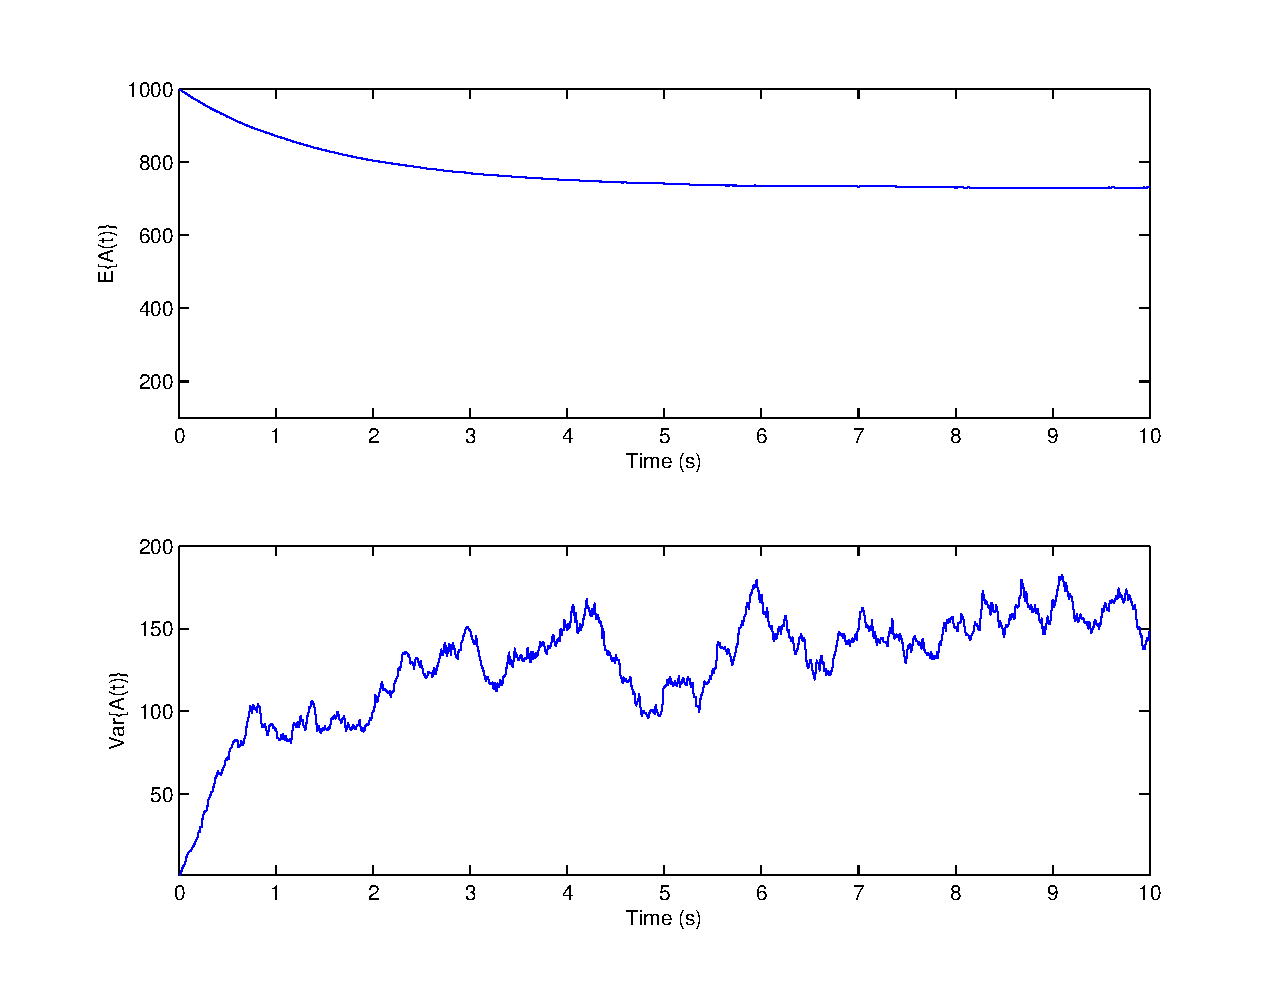
\includegraphics[width=6in]{Tutorials/MatlabPlot.eps}}
\caption{Mean and variance of A(t) for the reaction $A + B \xrightleftharpoons[]{} C$.}
\label{fig:MatlabPlot}
\end{figure}

The resulting plot should look like that shown in \Figure{fig:MatlabPlot}.\\

As another example, we calculate some statistics about the distribution of the molecules in \abr{RDME} simulations. The lattice is stored as a four dimensional matrix with dimensions $x{\times}y{\times}z{\times}particlesPerSite$. In our example above, the number of particles per site was limited to eight. We will count the number of particles in any sites' first, second, third, etc position. Such a calculation can give an indication of how close the lattice is to overflowing.

{\small\begin{verbatim}
replicate=1;
L=permute(h5read('bimol-rdme.lm',sprintf('/Model/Diffusion/Lattice')),[4,3,2,1]);
psum=sum(sum(sum(L>0)));
disp(sprintf('initial=%d (%d %d %d %d %d %d %d %d) %d--%d',...
             sum(sum(sum(sum(L>0)))),psum,min(min(min(min(L)))),...
             max(max(max(max(L))))));
for ts=[0:100]
    L=permute(h5read('bimol-rdme.lm',...
             sprintf('/Simulations/%07d/Lattice/%010d',...
             replicate,ts)),[4:-1:1]);
    psum=sum(sum(sum(L>0)));
    disp(sprintf('ts %4d=%d (%d %d %d %d %d %d %d %d) %d--%d',ts,...
             sum(sum(sum(sum(L>0)))),psum,min(min(min(min(L)))),...
             max(max(max(max(L))))));
end
\end{verbatim}}

Note that here again we used the \file{permute(hdf5read(...),[4,3,2,1])} command to reorder the 4D matrices to column major format after the data was loaded.\\

\subsection{Visualizing a trajectory using VMD}

If you have installed the VMD plugin, you can use VMD to visualize \abr{RDME} trajectories. For general instructions on using VMD, please see the VMD help at \url{http://www.ks.uiuc.edu/Research/vmd/}. Here we will focus on using VMD to visualize Lattice Microbes trajectories. First, ensure that your VMD plugin is functioning by starting VMD and then checking the VMD console for a message like:

{\small\begin{verbatim}
LMplugin Info) version 2 build by XXXXXXXX on XXX at XXXX-XX-XX XX:XX:XX
\end{verbatim}}

\begin{figure}
\centerline{\includegraphics[width=4in]{Tutorials/VMDOpen.png}}
\caption{VMD open file dialog.}
\label{fig:VMDOpen}
\end{figure}

Next, go to the menu and choose \gui{File$\rightarrow$New Molecule...}. Select \gui{Lattice Microbes} in the \gui{Determine file type:} drop down and browse to the file \file{bimol-rdme.lm}. Finally, press the \gui{Load} button (see \Figure{fig:VMDOpen}).\\

The trajectory should load with 101 frames. Initially, the VMD \gui{OpenGL} display will show only small points for each molecule. Change the representation by choosing \gui{Graphics$\rightarrow$Representations...} from the menu and then changing the \gui{Drawing Method} drop down to be \gui{VDW}. Now the molecules should appear as spheres. Next, change the \gui{Coloring Method} drop down to be \gui{Type} and molecules of different types should appear in different colors, as shown in \Figure{fig:VMDMolecules}. Press the triangular play button to play the simulation trajectory.\\

\begin{figure}
\centerline{\includegraphics[width=4in]{Tutorials/VMDMolecules.png}}
\caption{VMD molecule display.}
\label{fig:VMDMolecules}
\end{figure}

Finally, you may use the \gui{Selected Atoms} text field in the \gui{Graphical Representations} dialog to change which molecules are displayed. Change the text from ``\file{all}'' to ``\file{name particle and type 1}'' to show only A molecules. Likewise you can use ``\file{name particle and type 2}'' and ``\file{name particle and type 3}'' to view molecules of type B and C respectively.




\subsection{Importing an SBML reaction model}

Finally, we will show how you can use SBML files to set the reaction model, in addition to specifying the reaction matrices as shown above. First, copy the following SBML text into a file named \file{bimol.sbml}

{\small\begin{verbatim}
<?xml version="1.0" encoding="UTF-8"?>
<sbml xmlns="http://www.sbml.org/sbml/level3/version1/core" level="3" version="1">
    <model id="bimolecular" substanceUnits="item" timeUnits="second"
           volumeUnits="litre" extentUnits="item">
        <listOfUnitDefinitions>
            <unitDefinition id="per_second">
                <listOfUnits>
                    <unit kind="second" exponent="-1" scale="0" multiplier="1"/>
                </listOfUnits>
            </unitDefinition>
            <unitDefinition id="per_item_per_second">
                <listOfUnits>
                    <unit kind="item"   exponent="-1" scale="0" multiplier="1"/>
                    <unit kind="second" exponent="-1" scale="0" multiplier="1"/>
                </listOfUnits>
            </unitDefinition>
            <unitDefinition id="per_molar_per_second">
                <listOfUnits>
                    <unit kind="litre"  exponent="1" scale="0" multiplier="1"/>
                    <unit kind="mole"   exponent="-1" scale="0" multiplier="1"/>
                    <unit kind="second" exponent="-1" scale="0" multiplier="1"/>
                </listOfUnits>
            </unitDefinition>
        </listOfUnitDefinitions>
        <listOfCompartments>
            <compartment id="cell" size="1e-15" spatialDimensions="3"
                         constant="true"/>
        </listOfCompartments>
        <listOfSpecies>
            <species id="A" compartment="cell" initialAmount="1000"
                     hasOnlySubstanceUnits="true" boundaryCondition="false"
                     constant="false"/>
            <species id="B" compartment="cell" initialAmount="1000"
                     hasOnlySubstanceUnits="true" boundaryCondition="false"
                     constant="false"/>
            <species id="C" compartment="cell" initialAmount="0"
                     hasOnlySubstanceUnits="true" boundaryCondition="false"
                     constant="false"/>
        </listOfSpecies>
        <listOfReactions>
            <reaction id="Forward" reversible="false" fast="false">
                <listOfReactants>
                    <speciesReference species="A" stoichiometry="1"
                                      constant="true"/>
                    <speciesReference species="B" stoichiometry="1"
                                      constant="true"/>
                </listOfReactants>
                <listOfProducts>
                    <speciesReference species="C" stoichiometry="1"
                                      constant="true"/>
                </listOfProducts>
                <kineticLaw>
                    <math xmlns="http://www.w3.org/1998/Math/MathML">
                        <apply>
                            <divide/>
                            <apply>
                                <times/>
                                <ci> k1 </ci>
                                <ci> A </ci>
                                <ci> B </ci>
                            </apply>
                            <apply>
                                <times/>
                                <csymbol encoding="text"
                      definitionURL="http://www.sbml.org/sbml/symbols/avogadro"/>
                                <ci> cell </ci>
                            </apply>
                        </apply>
                    </math>
                    <listOfLocalParameters>
                        <localParameter id="k1" value="1.07e5"
                                        units="per_molar_per_second"/>
                    </listOfLocalParameters>
                </kineticLaw>
            </reaction>
            <reaction id="Reverse" reversible="false" fast="false">
                <listOfReactants>
                    <speciesReference species="C" stoichiometry="1"
                    constant="true"/>
                </listOfReactants>
                <listOfProducts>
                    <speciesReference species="A" stoichiometry="1"
                                      constant="true"/>
                    <speciesReference species="B" stoichiometry="1"
                                      constant="true"/>
                </listOfProducts>
                <kineticLaw>
                    <math xmlns="http://www.w3.org/1998/Math/MathML">
                        <apply>
                            <times/>
                            <ci> k2 </ci>
                            <ci> C </ci>
                        </apply>
                    </math>
                    <listOfLocalParameters>
                        <localParameter id="k2" value="0.351" units="per_second"/>
                    </listOfLocalParameters>
                </kineticLaw>
            </reaction>
        </listOfReactions>
    </model>
</sbml>
\end{verbatim}}

Next, create a simulation file from the SBML file:
{\small\begin{verbatim}
[user@host qs/bimol]$ lm_sbml_import bimol-cme-sbml.lm bimol.sbml
\end{verbatim}}

The reaction model is now ready to be simulated:
{\small\begin{verbatim}
[user@host qs/bimol]$ lm_setp bimol-cme-sbml.lm writeInterval=1e-3 maxTime=1e1
[user@host qs/bimol]$ lm -r 1-100 -ws -f bimol-cme-sbml.lm
\end{verbatim}}


                                                               

\chapter{Quick-Start Guide}

\section{Simulating a bimolecular reaction}

As a simple first example, we will consider the reversible bimolecular reaction $A + B \xrightleftharpoons[k_{2}]{k_{1}} C$. We will simulate two variations of this reaction, one it which the molecules are assumed to move very quickly relative to the reaction rate (``well-stirred'') and one in which the diffusion rates do play a significant role in the reacting system. We will solve these two models using \abr{CME} and \abr{RDME} sampling methods, respectively.\\

The overall steps involved will be as follows:
\begin{enumerate}
\item Build the simulation files containing the reaction and diffusion models.
\item Run the simulations using any solver specific parameters.
\item Analyze the simulation output. Output is saved directly into the simulation file.
\end{enumerate}

To begin, open a terminal and change to the \file{qs/bimol} directory in your User's Guide installation.

\subsection{Building the models}

The most straightforward way to construct a reaction model for a Lattice Microbes simulation is to directly set the matrices in the simulation file. The utilities \file{lm\_setrm} and \file{lm\_setdm} allow one to set the matrices for the reaction and diffusion models, respectively. The details of the matrices themselves will be described elsewhere. For the bimolecular reaction described above with $k1=\scimath{1.07}{5}\,M^{-1}\,s^{-1}$ and $k2=0.351\,s^{-1}$, we use the following command to build the reaction model:
{\small\begin{verbatim}
[user@host qs/bimol]$ lm_setrm bimol-cme.lm numberSpecies=3 numberReactions=2 \
                    "InitialSpeciesCounts=[1000,1000,0]" "ReactionTypes=[2,1]" \
                    "ReactionRateConstants(:,0)=[1.78e-4;0.351]" \
                    "StoichiometricMatrix=[-1,1;-1,1;1,-1]" \
                    "DependencyMatrix=[1,0;1,0;0,1]"
\end{verbatim}}

Note that we used the relationship between the stochastic and deterministic second order rate constants $k2'=k2/N_A{\cdot}V$ with a simulation volume of $V=\scimath{1}{-15}\,L$ to obtain the rate constant for the model. The file \file{bimol-cme.lm} is now ready to be simulated using the \abr{CME}.\\

Since the reaction portion of an \abr{RDME} model is identical to the \abr{CME} model, we simply copy the reaction model to a new simulation file and then set the diffusion matrices on the new file. Here, we use a diffusion coefficient $D=\scimath{1}{-14}\,m^2\,s{-1}$ for all molecules and a $32{\times}32{\times}32$ lattice with a spacing of $\lambda=\scimath{31.25}{-9}\,m$.
{\small\begin{verbatim}
[user@host qs/bimol]$ cp bimol-cme.lm bimol-rdme.lm
[user@host qs/bimol]$ lm_setdm bimol-rdme.lm numberReactions=2 numberSpecies=3 \
                    numberSiteTypes=1 "latticeSize=[32,32,32]" \
                    latticeSpacing=31.25e-9 particlesPerSite=8 \
                    "DiffusionMatrix=[1e-14]" "ReactionLocationMatrix=[1]"
\end{verbatim}}

The file \file{bimol-rdme.lm} is now ready to be simulated using the \abr{RDME}.

\subsection{Running the simulations}

\subsubsection{Sampling the CME using the Gillespie direct method}

To simulate the well-stirred version of the bimolecular reaction model, we will use the Gillespie direct method, which is the default method for well-stirred simulations in Lattice Microbes. Before we run the simulations, we first set a few simulation parameters for the solver. The \file{lm\_setp} utility allows one to set solver specific parameters in the simulation file. Here, we tell the solver to simulate for 10 seconds and write out the system state every 0.001 second.
{\small\begin{verbatim}
[user@host qs/bimol]$ lm_setp bimol-cme.lm writeInterval=1e-3 maxTime=1e1
\end{verbatim}}

Finally, we run the actual simulation itself:
{\small\begin{verbatim}
[user@host qs/bimol]$ lm -r 1-100 -ws -f bimol-cme.lm
\end{verbatim}}
The \file{-r} option tells the solver to simulate replicates 1--100 and the \file{-ws} option tells Lattice Microbes to use the default well-stirred solver. Following completion of the runs the \file{bimol-cme.lm} file will contain the sampling data for all of the simulation replicates.

\subsubsection{Sampling the RDME using the next-subvolume method}

If no \abrs{GPU} are attached to your computer, the only available \abr{RDME} solver is the next-subvolume method. We first set the appropriate parameters as before, but additionally, since we wish to track individual molecules, we must set a lattice output interval. Writing the lattice too frequently can consume an enormous amount of disk space so one should sample the lattice much less frequently than the system state, which only outputs the total count of each molecule type. Here, we sample the lattice every 0.1 second so we will have 100 samples of each 10 second simulation replicate.
{\small\begin{verbatim}
[user@host qs/bimol]$ lm_setp bimol-rdme.lm writeInterval=1e-3 \
                    latticeWriteInterval=1e-1 maxTime=1e1
\end{verbatim}}

We then run the \abr{RDME} simulations. These simulations take significantly longer than the well-stirred equivalents, so here we only simulate 10 replicates:
{\small\begin{verbatim}
[user@host qs/bimol]$ lm -r 1-10 -sl lm::rdme::NextSubvolumeSolver \
                    -f bimol-rdme.lm
\end{verbatim}}

All of the system state information and lattice data for every replicate will be saved into the \file{bimol-cme.lm} file.

\subsubsection{Sampling the RDME using the MPD-RDME method}

If you do have an NVIDIA \abr{GPU} attached to your computer, you can also use the MPD-RDME solver. This is an approximate RDME solver that uses a time stepping approach to dramatically increase simulation performance. We will run ten additional RDME replicates using the MPD-RDME. First, set the time step parameter to 3 milliseconds:
{\small\begin{verbatim}
[user@host qs/bimol]$ lm_setp bimol-rdme.lm timestep=3.0e-3
\end{verbatim}}

Then run replicates 11-20 using the MPD-RDME solver:
{\small\begin{verbatim}
[user@host qs/bimol]$ lm -r 11-20 -sl lm::rdme::MpdRdmeSolver -f bimol-rdme.lm
\end{verbatim}}

Following completion of the runs, ten additional simulation replicates will have been added to the \file{bimol-cme.lm} file.

\subsection{Looking at the simulation output}

\begin{figure}
\centerline{\includegraphics[width=4in]{Tutorials/HDFViewOpen.png}}
\caption{HDFView showing an open Lattice Microbes simulation file.}
\label{fig:HDFViewOpen}
\end{figure}

The output data is stored in a Lattice Microbes simulation file, which is an HDF5 encoded file that stores large, independent data sets in a hierarchical structure. To view the data, one must use an HDF5 viewer such as HDFView available at:\\
\url{http://www.hdfgroup.org/hdf-java-html/hdfview/}\\

To install the HDFView program, please follow the installation instructions for your platform.

\subsubsection{Opening a simulation file}

To open a Lattice Microbes simulation file in HDFView choose \gui{File$\rightarrow$Open} from the menu. Navigate to your \file{qs/bimol} directory in the \gui{Open} dialog. Be sure to change the \gui{Files of Type:} option to \gui{All Files} and then select the \file{bimol-cme.lm} file.\\

Once the file is opened, the individual folders containing the \gui{Model}, \gui{Parameters}, and \gui{Simulation} data can be expanded, as shown in \Figure{fig:HDFViewOpen}. Datasets are shown as small grid-like icons underneath the folders. Double clicking on a dataset will display its contents in the viewer panel to the right. For additional usage details, please see the HDFView User's Guide, located on the download page given above.


\subsubsection{Overview of the file format}

Lattice Microbes simulation files are organized into three top level folders: \gui{Model}, \gui{Parameters}, and \gui{Simulation}.\\

The \gui{Model} folder contains two subfolders for the \gui{Reaction} and \gui{Diffusion} models, as needed for the simulation. Each folder has several attributes and contains several datasets corresponding to the matrices that describe the model. Further details of the matrices themselves are provided elsewhere.\\

The \gui{Parameters} folder acts as a collection point for solver specific parameters, which are set as attributes on the folder. Details of individual parameters are provided elsewhere.\\

The \gui{Simulations} folder contains the actual output from the simulations. Beneath the folder is one folder for each simulation replicate, numbered accordingly. For each simulation replicate the data is stored in a variety of matrices and folders, which are specific to the simulation method.

\subsection{Analyzing a simulation using Matlab}

The HDF5 file format used by the Lattice Microbes software can be directly read by Matlab, easing the analysis of simulation data. Here, we will calculate the probability as a function of time for the system to have a specific number of A molecules, {\ie}, $P_A(t)$. We will use this \abr{PDF} to calculate the mean and variance as a function of time.\\

First, we load the number of A molecules for each replicate at each time point from the simulation file and transform the counts into a \abr{PDF}:
{\small\begin{verbatim}
inputFilename='bimol-cme.lm';
x=[0:1000];
numberReplicates=100;
species=1;
for R=[1:numberReplicates]
    if R == 1
        ts=cast(permute(hdf5read(inputFilename,...
           sprintf('/Simulations/%07d/SpeciesCountTimes',R)),[2,1]),'double');
        Pt=zeros(size(x,2),size(ts,2));
    end
    counts=cast(permute(hdf5read(inputFilename,...
           sprintf('/Simulations/%07d/SpeciesCounts',R)),[2,1]),'double');
    for ti=[1:size(ts,2)]
        Pt(counts(ti,species)+1,ti)=Pt(counts(ti,species)+1,ti)+1;
    end
end
Pt=Pt./numberReplicates;
\end{verbatim}}

Note that HDF5 files store data in row major format while Matlab stores data in column major format. In the above Matlab code, we used the \file{permute(hdf5read(...),[2,1])} command to reorder the 2D matrices to column major format after the data was loaded.\\

Next, we calculate the mean and variance from the $P_A(t)$:
{\small\begin{verbatim}
E=zeros(1,size(ts,2));
V=zeros(1,size(ts,2));
for ti=[1:size(ts,2)]
    E(ti)=sum(x'.*Pt(:,ti));
    V(ti)=sum((power(x'-E(ti),2)).*Pt(:,ti));
end
\end{verbatim}}

Finally, we plot the mean and variance as a function of time:
{\small\begin{verbatim}
subplot(2,1,1);
plot(ts(1:10:end), E(1:10:end));
axis([0 10 1e2 1e3]); xlabel('Time (s)'); ylabel('E\{A(t)\}');
subplot(2,1,2);
plot(ts(1:10:end), V(1:10:end));
axis([0 10 1e0 2e2]); xlabel('Time (s)'); ylabel('Var\{A(t)\}');
\end{verbatim}}

\begin{figure}
\centerline{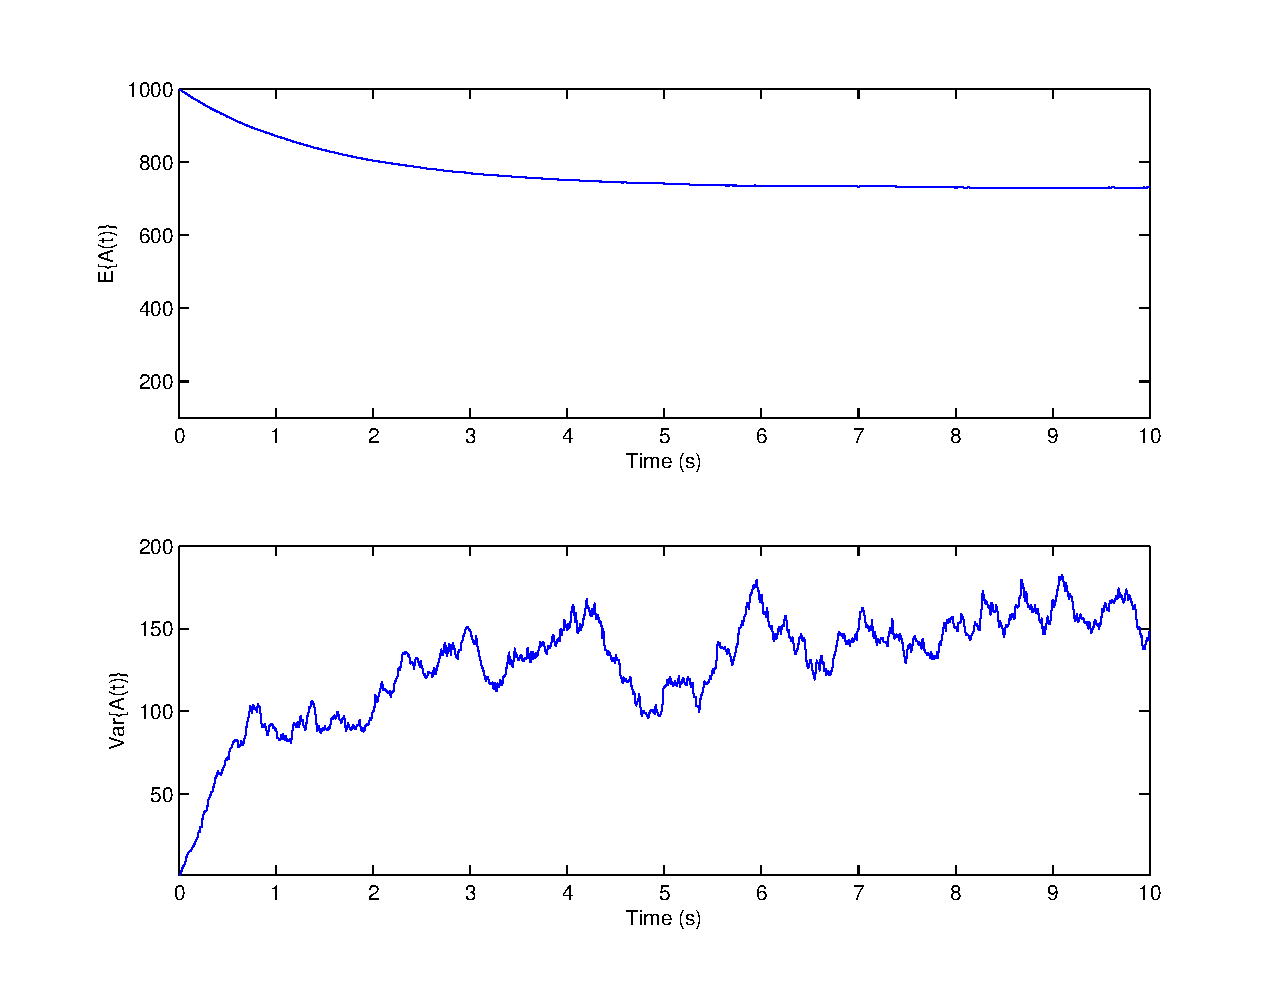
\includegraphics[width=6in]{Tutorials/MatlabPlot.eps}}
\caption{Mean and variance of A(t) for the reaction $A + B \xrightleftharpoons[]{} C$.}
\label{fig:MatlabPlot}
\end{figure}

The resulting plot should look like that shown in \Figure{fig:MatlabPlot}.\\

As another example, we calculate some statistics about the distribution of the molecules in \abr{RDME} simulations. The lattice is stored as a four dimensional matrix with dimensions $x{\times}y{\times}z{\times}particlesPerSite$. In our example above, the number of particles per site was limited to eight. We will count the number of particles in any sites' first, second, third, etc position. Such a calculation can give an indication of how close the lattice is to overflowing.

{\small\begin{verbatim}
replicate=1;
L=permute(h5read('bimol-rdme.lm',sprintf('/Model/Diffusion/Lattice')),[4,3,2,1]);
psum=sum(sum(sum(L>0)));
disp(sprintf('initial=%d (%d %d %d %d %d %d %d %d) %d--%d',...
             sum(sum(sum(sum(L>0)))),psum,min(min(min(min(L)))),...
             max(max(max(max(L))))));
for ts=[0:100]
    L=permute(h5read('bimol-rdme.lm',...
             sprintf('/Simulations/%07d/Lattice/%010d',...
             replicate,ts)),[4:-1:1]);
    psum=sum(sum(sum(L>0)));
    disp(sprintf('ts %4d=%d (%d %d %d %d %d %d %d %d) %d--%d',ts,...
             sum(sum(sum(sum(L>0)))),psum,min(min(min(min(L)))),...
             max(max(max(max(L))))));
end
\end{verbatim}}

Note that here again we used the \file{permute(hdf5read(...),[4,3,2,1])} command to reorder the 4D matrices to column major format after the data was loaded.\\

\subsection{Visualizing a trajectory using VMD}

If you have installed the VMD plugin, you can use VMD to visualize \abr{RDME} trajectories. For general instructions on using VMD, please see the VMD help at \url{http://www.ks.uiuc.edu/Research/vmd/}. Here we will focus on using VMD to visualize Lattice Microbes trajectories. First, ensure that your VMD plugin is functioning by starting VMD and then checking the VMD console for a message like:

{\small\begin{verbatim}
LMplugin Info) version 2 build by XXXXXXXX on XXX at XXXX-XX-XX XX:XX:XX
\end{verbatim}}

\begin{figure}
\centerline{\includegraphics[width=4in]{Tutorials/VMDOpen.png}}
\caption{VMD open file dialog.}
\label{fig:VMDOpen}
\end{figure}

Next, go to the menu and choose \gui{File$\rightarrow$New Molecule...}. Select \gui{Lattice Microbes} in the \gui{Determine file type:} drop down and browse to the file \file{bimol-rdme.lm}. Finally, press the \gui{Load} button (see \Figure{fig:VMDOpen}).\\

The trajectory should load with 101 frames. Initially, the VMD \gui{OpenGL} display will show only small points for each molecule. Change the representation by choosing \gui{Graphics$\rightarrow$Representations...} from the menu and then changing the \gui{Drawing Method} drop down to be \gui{VDW}. Now the molecules should appear as spheres. Next, change the \gui{Coloring Method} drop down to be \gui{Type} and molecules of different types should appear in different colors, as shown in \Figure{fig:VMDMolecules}. Press the triangular play button to play the simulation trajectory.\\

\begin{figure}
\centerline{\includegraphics[width=4in]{Tutorials/VMDMolecules.png}}
\caption{VMD molecule display.}
\label{fig:VMDMolecules}
\end{figure}

Finally, you may use the \gui{Selected Atoms} text field in the \gui{Graphical Representations} dialog to change which molecules are displayed. Change the text from ``\file{all}'' to ``\file{name particle and type 1}'' to show only A molecules. Likewise you can use ``\file{name particle and type 2}'' and ``\file{name particle and type 3}'' to view molecules of type B and C respectively.




\subsection{Importing an SBML reaction model}

Finally, we will show how you can use SBML files to set the reaction model, in addition to specifying the reaction matrices as shown above. First, copy the following SBML text into a file named \file{bimol.sbml}

{\small\begin{verbatim}
<?xml version="1.0" encoding="UTF-8"?>
<sbml xmlns="http://www.sbml.org/sbml/level3/version1/core" level="3" version="1">
    <model id="bimolecular" substanceUnits="item" timeUnits="second"
           volumeUnits="litre" extentUnits="item">
        <listOfUnitDefinitions>
            <unitDefinition id="per_second">
                <listOfUnits>
                    <unit kind="second" exponent="-1" scale="0" multiplier="1"/>
                </listOfUnits>
            </unitDefinition>
            <unitDefinition id="per_item_per_second">
                <listOfUnits>
                    <unit kind="item"   exponent="-1" scale="0" multiplier="1"/>
                    <unit kind="second" exponent="-1" scale="0" multiplier="1"/>
                </listOfUnits>
            </unitDefinition>
            <unitDefinition id="per_molar_per_second">
                <listOfUnits>
                    <unit kind="litre"  exponent="1" scale="0" multiplier="1"/>
                    <unit kind="mole"   exponent="-1" scale="0" multiplier="1"/>
                    <unit kind="second" exponent="-1" scale="0" multiplier="1"/>
                </listOfUnits>
            </unitDefinition>
        </listOfUnitDefinitions>
        <listOfCompartments>
            <compartment id="cell" size="1e-15" spatialDimensions="3"
                         constant="true"/>
        </listOfCompartments>
        <listOfSpecies>
            <species id="A" compartment="cell" initialAmount="1000"
                     hasOnlySubstanceUnits="true" boundaryCondition="false"
                     constant="false"/>
            <species id="B" compartment="cell" initialAmount="1000"
                     hasOnlySubstanceUnits="true" boundaryCondition="false"
                     constant="false"/>
            <species id="C" compartment="cell" initialAmount="0"
                     hasOnlySubstanceUnits="true" boundaryCondition="false"
                     constant="false"/>
        </listOfSpecies>
        <listOfReactions>
            <reaction id="Forward" reversible="false" fast="false">
                <listOfReactants>
                    <speciesReference species="A" stoichiometry="1"
                                      constant="true"/>
                    <speciesReference species="B" stoichiometry="1"
                                      constant="true"/>
                </listOfReactants>
                <listOfProducts>
                    <speciesReference species="C" stoichiometry="1"
                                      constant="true"/>
                </listOfProducts>
                <kineticLaw>
                    <math xmlns="http://www.w3.org/1998/Math/MathML">
                        <apply>
                            <divide/>
                            <apply>
                                <times/>
                                <ci> k1 </ci>
                                <ci> A </ci>
                                <ci> B </ci>
                            </apply>
                            <apply>
                                <times/>
                                <csymbol encoding="text"
                      definitionURL="http://www.sbml.org/sbml/symbols/avogadro"/>
                                <ci> cell </ci>
                            </apply>
                        </apply>
                    </math>
                    <listOfLocalParameters>
                        <localParameter id="k1" value="1.07e5"
                                        units="per_molar_per_second"/>
                    </listOfLocalParameters>
                </kineticLaw>
            </reaction>
            <reaction id="Reverse" reversible="false" fast="false">
                <listOfReactants>
                    <speciesReference species="C" stoichiometry="1"
                    constant="true"/>
                </listOfReactants>
                <listOfProducts>
                    <speciesReference species="A" stoichiometry="1"
                                      constant="true"/>
                    <speciesReference species="B" stoichiometry="1"
                                      constant="true"/>
                </listOfProducts>
                <kineticLaw>
                    <math xmlns="http://www.w3.org/1998/Math/MathML">
                        <apply>
                            <times/>
                            <ci> k2 </ci>
                            <ci> C </ci>
                        </apply>
                    </math>
                    <listOfLocalParameters>
                        <localParameter id="k2" value="0.351" units="per_second"/>
                    </listOfLocalParameters>
                </kineticLaw>
            </reaction>
        </listOfReactions>
    </model>
</sbml>
\end{verbatim}}

Next, create a simulation file from the SBML file:
{\small\begin{verbatim}
[user@host qs/bimol]$ lm_sbml_import bimol-cme-sbml.lm bimol.sbml
\end{verbatim}}

The reaction model is now ready to be simulated:
{\small\begin{verbatim}
[user@host qs/bimol]$ lm_setp bimol-cme-sbml.lm writeInterval=1e-3 maxTime=1e1
[user@host qs/bimol]$ lm -r 1-100 -ws -f bimol-cme-sbml.lm
\end{verbatim}}


                                                               


% References
\newpage
\addcontentsline{toc}{chapter}{Bibliography}
\bibliographystyle{inorder}
\bibliography{references,zlsgroup-2011}

\end{document}


